\documentclass[12pt,a4paper]{article}
\usepackage{amsmath, amssymb, geometry, booktabs, xcolor, hyperref,
            listings, pgfplots, tcolorbox, enumitem, fancyhdr, tikz, array}
\usepgfplotslibrary{fillbetween}
\geometry{margin=2.5cm}
\pgfplotsset{compat=1.18}
\tcbuselibrary{skins, breakable}

% Define custom environments
\newtcolorbox{curiositybox}[1]{colback=yellow!10, colframe=orange!80, title=#1, breakable}
\newtcolorbox{infobox}[1]{colback=blue!5, colframe=blue!60, title=#1, breakable}
\newtcolorbox{mistakebox}[1]{colback=red!5, colframe=red!60, title=#1, breakable}
\newtcolorbox{learnbox}[1]{colback=green!5, colframe=green!60, title=#1, breakable}

% Header and Footer
\pagestyle{fancy}
\fancyhf{}
\lhead{Differential Geometry and Fields}
\rhead{Unit 4 -- LAC}
\cfoot{\thepage}

% Document Title Setup
\title{\textbf{Differential Geometry and Fields} \\ \large Unit 4 -- Multivariable Differentiation and Optimization}
\author{Department of Mathematics}
\date{\today}

\begin{document}
\maketitle
\tableofcontents
\newpage

%==============================================================
\section{Real-World Engineering Hook}
%==============================================================

\begin{curiositybox}{Why Should an Engineer Care?}
\textbf{Scenario 1 --- Electromagnetics:} The gradient of electric potential $V$ gives the electric field $\mathbf{E} = -\nabla V$. In finite element analysis of a capacitor, if the gradient is computed incorrectly, the field distribution is wrong and the device fails its design specification. Every voltage-to-field conversion in circuit simulation relies on this gradient relationship.

\vspace{6pt}
\textbf{Scenario 2 --- Fluid Mechanics (CFD):} A computational fluid dynamics engineer models airflow around an aerofoil. The divergence of the velocity field $\mathbf{V}$ must equal zero ($\nabla \cdot \mathbf{V} = 0$) for incompressible flow. If a non-zero divergence leaks into the numerical mesh, mass is artificially created or destroyed at every time step, rendering the entire simulation physically invalid.

\vspace{6pt}
\textbf{Scenario 3 --- Structural Analysis:} The normal to a surface defines the direction along which contact loads are applied in a finite element model. Computing the tangent plane incorrectly at a contact patch propagates errors into contact stress calculations, which can lead to under-designed components and fatigue failure.

\vspace{6pt}
\textbf{Scenario 4 --- Heat Transfer:} The directional derivative of a temperature field $T(\mathbf{r})$ gives the rate of heat flux in any chosen direction. Thermal engineers use this to optimise cooling fin geometry --- identifying the direction of maximum heat flow and placing fin material accordingly.
\end{curiositybox}

%==============================================================
\section{Why This Topic Exists}
%==============================================================

\begin{center}
\begin{tabular}{>{\bfseries}p{4.5cm} p{9.5cm}}
\toprule
Theoretical Concept & Engineering Application / Consequence of Misunderstanding \\
\midrule
Gradient \& Directional Derivative &
Electric field from potential ($\mathbf{E} = -\nabla V$); direction of steepest temperature rise in thermal analysis. An incorrect gradient yields the wrong field direction, causing device failure or incorrect thermal management. \\[6pt]
Tangent Plane \& Normal Line &
Contact stress analysis and surface meshing in FEM. A wrong normal vector means loads are applied in the incorrect direction, introducing structural errors that can cause fatigue failure. \\[6pt]
Divergence \& Curl &
CFD incompressibility ($\nabla \cdot \mathbf{V} = 0$), electromagnetic Gauss's law ($\nabla \cdot \mathbf{E} = \rho/\varepsilon_0$), and irrotational potential flow. A non-zero spurious divergence destroys mass conservation in a simulation; a missed curl component hides vorticity. \\
\bottomrule
\end{tabular}
\end{center}

\vspace{10pt}

\begin{learnbox}{Core Learning Objectives}
By the end of this topic you will be able to:
\begin{itemize}[leftmargin=*]
  \item Compute the gradient $\nabla f$ of a scalar field in three dimensions and evaluate it at a given point.
  \item Calculate the directional derivative of a scalar field in any specified direction using the unit vector formula.
  \item Write the tangent plane equation and parametric normal line for an implicit surface $F(x,y,z) = 0$.
  \item Compute the divergence $\nabla \cdot \mathbf{F}$ and curl $\nabla \times \mathbf{F}$ of a vector field.
  \item Classify a vector field as solenoidal, irrotational, both, or neither.
  \item Find a scalar potential $\varphi$ for an irrotational field by successive integration.
\end{itemize}
\end{learnbox}

%==============================================================
\section{Intuition First and Mathematical Definitions}
%==============================================================

\subsection{Gradient and Directional Derivative}

Imagine the scalar field $f(x,y,z)$ as a mountain landscape where the value of $f$ gives the altitude at each point. The gradient $\nabla f$ is like a compass needle that always points in the direction of steepest uphill climb. Its magnitude tells you exactly how steep that slope is. The directional derivative generalises this idea: it answers the question ``how fast does altitude change if I walk in some arbitrary direction $\mathbf{u}$?'' and the answer is simply the projection of the gradient onto that direction.

\begin{infobox}{Gradient and Directional Derivative --- Formal Definitions}
Let $f(x,y,z)$ be a differentiable scalar field.

\textbf{Gradient:}
\[
  \nabla f = \frac{\partial f}{\partial x}\,\mathbf{i} + \frac{\partial f}{\partial y}\,\mathbf{j} + \frac{\partial f}{\partial z}\,\mathbf{k}
\]

\textbf{Properties of the Gradient:}
\begin{itemize}[leftmargin=*]
  \item $\nabla f$ points in the direction of \emph{steepest ascent} of $f$.
  \item $|\nabla f|$ equals the \emph{maximum rate of change} of $f$ at that point.
  \item $\nabla f$ is perpendicular (normal) to the level surface $f = c$ passing through the point.
  \item The direction of steepest descent is $-\nabla f$.
\end{itemize}

\textbf{Directional Derivative:}

For a unit vector $\hat{\mathbf{u}}$ (i.e., $|\hat{\mathbf{u}}| = 1$):
\[
  D_{\hat{\mathbf{u}}} f = \nabla f \cdot \hat{\mathbf{u}}
\]

If the direction is given as a non-unit vector $\mathbf{v}$, normalise first:
\[
  \hat{\mathbf{u}} = \frac{\mathbf{v}}{|\mathbf{v}|}
\]

\textbf{Key Extremes:}
\begin{itemize}[leftmargin=*]
  \item Maximum value of $D_{\hat{\mathbf{u}}} f$ is $|\nabla f|$, achieved when $\hat{\mathbf{u}} \parallel \nabla f$.
  \item Minimum value is $-|\nabla f|$, achieved when $\hat{\mathbf{u}}$ is anti-parallel to $\nabla f$.
  \item $D_{\hat{\mathbf{u}}} f = 0$ when $\hat{\mathbf{u}} \perp \nabla f$ (moving along the level surface).
\end{itemize}
\end{infobox}

\vspace{8pt}
\textbf{Worked Example 3.1.1} --- Gradient and Directional Derivative at a Point

Let $f(x,y,z) = x^2 y + yz^2$. Find $\nabla f$ at the point $P(1, 2, 1)$ and then compute the directional derivative at $P$ in the direction of $\mathbf{v} = (1, 1, 1)$.

\textbf{Step 1: Compute partial derivatives (general expressions).}
\[
  \frac{\partial f}{\partial x} = 2xy, \qquad
  \frac{\partial f}{\partial y} = x^2 + z^2, \qquad
  \frac{\partial f}{\partial z} = 2yz
\]

\textbf{Step 2: Evaluate at $P(1, 2, 1)$.}
\[
  f_x(1,2,1) = 2(1)(2) = 4, \quad
  f_y(1,2,1) = 1^2 + 1^2 = 2, \quad
  f_z(1,2,1) = 2(2)(1) = 4
\]
\[
  \nabla f\big|_P = 4\,\mathbf{i} + 2\,\mathbf{j} + 4\,\mathbf{k}
\]

\textbf{Step 3: Normalise direction vector $\mathbf{v} = (1,1,1)$.}
\[
  |\mathbf{v}| = \sqrt{1^2+1^2+1^2} = \sqrt{3}
\]
\[
  \hat{\mathbf{u}} = \frac{1}{\sqrt{3}}\,\mathbf{i} + \frac{1}{\sqrt{3}}\,\mathbf{j} + \frac{1}{\sqrt{3}}\,\mathbf{k}
\]

\textbf{Step 4: Compute directional derivative.}
\[
  D_{\hat{\mathbf{u}}} f = \nabla f \cdot \hat{\mathbf{u}}
    = 4 \cdot \frac{1}{\sqrt{3}} + 2 \cdot \frac{1}{\sqrt{3}} + 4 \cdot \frac{1}{\sqrt{3}}
    = \frac{10}{\sqrt{3}} = \frac{10\sqrt{3}}{3} \approx 5.77
\]

\textbf{Conclusion:} The directional derivative at $P$ in the direction $(1,1,1)$ is $\dfrac{10\sqrt{3}}{3}$.

\vspace{8pt}
\textbf{Worked Example 3.1.2} --- Direction of Maximum Rate of Increase

Let $g(x,y,z) = x^2 + y^2 - z$. Find the direction and value of the maximum rate of increase at $Q(1,1,2)$.

\textbf{Step 1: Compute partial derivatives.}
\[
  \frac{\partial g}{\partial x} = 2x, \quad \frac{\partial g}{\partial y} = 2y, \quad \frac{\partial g}{\partial z} = -1
\]

\textbf{Step 2: Evaluate at $Q(1,1,2)$.}
\[
  \nabla g\big|_Q = 2(1)\,\mathbf{i} + 2(1)\,\mathbf{j} + (-1)\,\mathbf{k} = 2\,\mathbf{i} + 2\,\mathbf{j} - \mathbf{k}
\]

\textbf{Step 3: Direction of maximum increase is $\nabla g$ itself.}
\[
  \text{Direction} = (2, 2, -1)
\]

\textbf{Step 4: Maximum rate of change.}
\[
  |\nabla g| = \sqrt{4 + 4 + 1} = \sqrt{9} = 3
\]

\textbf{Conclusion:} The maximum rate of increase of $g$ at $Q$ is $3$, achieved in the direction $(2, 2, -1)$.

%-------------------------------------------------------------------
\subsection{Tangent Plane and Normal Line to a Surface}

Just as a tangent line kisses a smooth curve at a single point while sharing its slope, a tangent plane kisses a smooth surface at a single point while sharing the local tilt in every direction. The normal line is the unique straight line passing through that contact point and perpendicular to the tangent plane --- and it turns out to point exactly in the direction of $\nabla F$, the gradient of the surface function.

\begin{infobox}{Tangent Plane and Normal Line --- Formal Definitions}
\textbf{Implicit Surface} $F(x,y,z) = 0$:

Let $(x_0, y_0, z_0)$ be a point on the surface and let $F_x, F_y, F_z$ denote the partial derivatives of $F$ evaluated at that point.

\textbf{Tangent Plane:}
\[
  F_x(x - x_0) + F_y(y - y_0) + F_z(z - z_0) = 0
\]

\textbf{Normal Line (parametric):}
\[
  x = x_0 + F_x\, t, \quad y = y_0 + F_y\, t, \quad z = z_0 + F_z\, t, \quad t \in \mathbb{R}
\]

\textbf{Geometric Significance:} $\nabla F = (F_x, F_y, F_z)$ is \emph{normal} to the surface $F = 0$ at the point. Both the tangent plane and normal line are completely determined by this gradient vector.

\textbf{Special Case --- Explicit Surface} $z = f(x,y)$:

Rewrite as $F(x,y,z) = f(x,y) - z = 0$, so $F_x = f_x$, $F_y = f_y$, $F_z = -1$. The tangent plane becomes:
\[
  z - z_0 = f_x(x_0,y_0)(x - x_0) + f_y(x_0,y_0)(y - y_0)
\]

\textbf{Sign Convention:} When $F_z \neq 0$, the normal direction $(F_x, F_y, F_z)$ with $F_z < 0$ (as in $F = f-z$) points \emph{downward} unless adjusted.
\end{infobox}

\vspace{8pt}
\textbf{Worked Example 3.2.1} --- Tangent Plane and Normal Line to a Sphere

Find the tangent plane and normal line to the surface $x^2 + y^2 + z^2 = 14$ at the point $(1, 2, 3)$.

\textbf{Step 1: Verify the point lies on the surface.}
\[
  1^2 + 2^2 + 3^2 = 1 + 4 + 9 = 14 \quad \checkmark
\]

\textbf{Step 2: Define $F(x,y,z) = x^2 + y^2 + z^2 - 14$. Compute partial derivatives.}
\[
  F_x = 2x, \quad F_y = 2y, \quad F_z = 2z
\]

\textbf{Step 3: Evaluate at $(1, 2, 3)$.}
\[
  F_x = 2(1) = 2, \quad F_y = 2(2) = 4, \quad F_z = 2(3) = 6
\]

\textbf{Step 4: Write the tangent plane.}
\[
  2(x-1) + 4(y-2) + 6(z-3) = 0
\]
\[
  2x - 2 + 4y - 8 + 6z - 18 = 0
\]
\[
  \boxed{2x + 4y + 6z = 28 \quad \Longrightarrow \quad x + 2y + 3z = 14}
\]

\textbf{Step 5: Write the normal line.}
\[
  x = 1 + 2t, \quad y = 2 + 4t, \quad z = 3 + 6t
\]

\textbf{Geometric Interpretation:} The normal direction $(2,4,6)$ or simplified $(1,2,3)$ is the position vector itself, confirming that for a sphere centred at the origin, the normal always points radially outward.

\vspace{8pt}
\textbf{Worked Example 3.2.2} --- Tangent Plane via Two Methods

Find the tangent plane to $z = x^2 + y^2$ at $(1, 1, 2)$ and confirm agreement between the explicit and implicit approaches.

\textbf{Method A --- Explicit form.}

Here $f(x,y) = x^2 + y^2$. Partial derivatives: $f_x = 2x$, $f_y = 2y$.

At $(1,1)$: $f_x = 2$, $f_y = 2$, $z_0 = 2$.
\[
  z - 2 = 2(x - 1) + 2(y - 1)
\]
\[
  z = 2x + 2y - 2
\]

\textbf{Method B --- Implicit form.}

Let $F(x,y,z) = x^2 + y^2 - z$. Then $F_x = 2x$, $F_y = 2y$, $F_z = -1$.

At $(1,1,2)$: $F_x = 2$, $F_y = 2$, $F_z = -1$.
\[
  2(x-1) + 2(y-1) + (-1)(z-2) = 0
\]
\[
  2x - 2 + 2y - 2 - z + 2 = 0 \quad \Longrightarrow \quad z = 2x + 2y - 2
\]

Both methods give $z = 2x + 2y - 2$. \textbf{The normal direction is $(2, 2, -1)$.}

%-------------------------------------------------------------------
\subsection{Divergence and Curl of a Vector Field}

Divergence asks ``is this point a source or a drain?'' --- imagine dropping a tiny ball of fluid into the field; if the fluid flows outward from the ball, divergence is positive (source); if it flows inward, divergence is negative (sink); if neither, the field is incompressible. Curl asks ``does this field spin things?'' --- imagine dropping a tiny paddle wheel into the field; if it rotates, the curl is non-zero. These two operations are the mathematical backbone of Maxwell's equations, Navier--Stokes equations, and virtually every physical field theory.

\begin{infobox}{Divergence and Curl --- Formal Definitions}
Let $\mathbf{F} = P\,\mathbf{i} + Q\,\mathbf{j} + R\,\mathbf{k}$ be a differentiable vector field.

\textbf{Divergence (scalar output):}
\[
  \nabla \cdot \mathbf{F} = \frac{\partial P}{\partial x} + \frac{\partial Q}{\partial y} + \frac{\partial R}{\partial z}
\]

\textbf{Curl (vector output):}
\[
  \nabla \times \mathbf{F} =
  \begin{vmatrix}
    \mathbf{i} & \mathbf{j} & \mathbf{k} \\
    \dfrac{\partial}{\partial x} & \dfrac{\partial}{\partial y} & \dfrac{\partial}{\partial z} \\[4pt]
    P & Q & R
  \end{vmatrix}
  = \left(\frac{\partial R}{\partial y} - \frac{\partial Q}{\partial z}\right)\mathbf{i}
  - \left(\frac{\partial R}{\partial x} - \frac{\partial P}{\partial z}\right)\mathbf{j}
  + \left(\frac{\partial Q}{\partial x} - \frac{\partial P}{\partial y}\right)\mathbf{k}
\]

\textbf{Physical Interpretation:}
\begin{itemize}[leftmargin=*]
  \item $\nabla \cdot \mathbf{F} > 0$: point is a \emph{source} (field lines emanate).
  \item $\nabla \cdot \mathbf{F} < 0$: point is a \emph{sink} (field lines converge).
  \item $\nabla \cdot \mathbf{F} = 0$ everywhere: $\mathbf{F}$ is \emph{solenoidal} (divergence-free, incompressible).
  \item $\nabla \times \mathbf{F} = \mathbf{0}$ everywhere: $\mathbf{F}$ is \emph{irrotational} (conservative); a scalar potential $\varphi$ exists with $\mathbf{F} = \nabla \varphi$.
\end{itemize}

\textbf{Key Vector Identities:}
\begin{enumerate}[leftmargin=*]
  \item For any scalar field $f$: $\nabla \times (\nabla f) = \mathbf{0}$ always (gradient fields are always irrotational).
  \item For any vector field $\mathbf{F}$: $\nabla \cdot (\nabla \times \mathbf{F}) = 0$ always (curl fields are always solenoidal).
\end{enumerate}
\end{infobox}

\vspace{8pt}
\textbf{Worked Example 3.3.1} --- Divergence and Curl of a General Field

Let $\mathbf{F} = x^2 y\,\mathbf{i} + yz^2\,\mathbf{j} + zx^2\,\mathbf{k}$. Compute $\nabla \cdot \mathbf{F}$ and $\nabla \times \mathbf{F}$.

Here $P = x^2 y$, $Q = yz^2$, $R = zx^2$.

\textbf{Step 1: Divergence.}
\[
  \frac{\partial P}{\partial x} = 2xy, \quad \frac{\partial Q}{\partial y} = z^2, \quad \frac{\partial R}{\partial z} = x^2
\]
\[
  \nabla \cdot \mathbf{F} = 2xy + z^2 + x^2
\]
Since this is not identically zero, $\mathbf{F}$ is \textbf{not solenoidal}.

\textbf{Step 2: Curl --- compute each component.}

$\mathbf{i}$-component: $\dfrac{\partial R}{\partial y} - \dfrac{\partial Q}{\partial z} = 0 - 2yz = -2yz$

$\mathbf{j}$-component: $-\!\left(\dfrac{\partial R}{\partial x} - \dfrac{\partial P}{\partial z}\right) = -(2xz - 0) = -2xz$

$\mathbf{k}$-component: $\dfrac{\partial Q}{\partial x} - \dfrac{\partial P}{\partial y} = 0 - x^2 = -x^2$

\[
  \nabla \times \mathbf{F} = -2yz\,\mathbf{i} - 2xz\,\mathbf{j} - x^2\,\mathbf{k}
\]

Since $\nabla \times \mathbf{F} \neq \mathbf{0}$, $\mathbf{F}$ is \textbf{not irrotational}.

\textbf{Conclusion:} $\mathbf{F}$ is neither solenoidal nor irrotational.

\vspace{8pt}
\textbf{Worked Example 3.3.2} --- Verifying Irrotational Field and Finding Scalar Potential

Verify that $\mathbf{F} = 2xyz\,\mathbf{i} + x^2 z\,\mathbf{j} + x^2 y\,\mathbf{k}$ is irrotational, then find the scalar potential $\varphi$ such that $\nabla \varphi = \mathbf{F}$.

Here $P = 2xyz$, $Q = x^2 z$, $R = x^2 y$.

\textbf{Step 1: Check curl.}

$\mathbf{i}$: $\dfrac{\partial R}{\partial y} - \dfrac{\partial Q}{\partial z} = x^2 - x^2 = 0$

$\mathbf{j}$: $-\!\left(\dfrac{\partial R}{\partial x} - \dfrac{\partial P}{\partial z}\right) = -(2xy - 2xy) = 0$

$\mathbf{k}$: $\dfrac{\partial Q}{\partial x} - \dfrac{\partial P}{\partial y} = 2xz - 2xz = 0$

\[
  \nabla \times \mathbf{F} = \mathbf{0} \quad \checkmark \quad \text{Field is irrotational.}
\]

\textbf{Step 2: Find $\varphi$ from $\partial \varphi/\partial x = P = 2xyz$.}
\[
  \varphi = \int 2xyz\, dx = x^2 yz + g(y, z)
\]

\textbf{Step 3: Use $\partial \varphi/\partial y = Q = x^2 z$.}
\[
  \frac{\partial}{\partial y}\bigl(x^2 yz + g(y,z)\bigr) = x^2 z + \frac{\partial g}{\partial y} = x^2 z
  \quad \Rightarrow \quad \frac{\partial g}{\partial y} = 0 \quad \Rightarrow \quad g = h(z)
\]

\textbf{Step 4: Use $\partial \varphi/\partial z = R = x^2 y$.}
\[
  \frac{\partial}{\partial z}\bigl(x^2 yz + h(z)\bigr) = x^2 y + h'(z) = x^2 y
  \quad \Rightarrow \quad h'(z) = 0 \quad \Rightarrow \quad h = C
\]

\[
  \boxed{\varphi = x^2 yz + C}
\]

\textbf{Worked Example 3.3.3} --- Engineering: Incompressible Velocity Field

Velocity field $\mathbf{V} = 2x\,\mathbf{i} - 2y\,\mathbf{j} + 0\,\mathbf{k}$. Verify it is solenoidal (incompressible) and compute its curl.

\textbf{Step 1: Divergence.}
\[
  \nabla \cdot \mathbf{V} = \frac{\partial(2x)}{\partial x} + \frac{\partial(-2y)}{\partial y} + \frac{\partial(0)}{\partial z}
  = 2 + (-2) + 0 = 0 \quad \checkmark
\]

The flow is \textbf{incompressible} (solenoidal).

\textbf{Step 2: Curl.} With $P = 2x$, $Q = -2y$, $R = 0$:

$\mathbf{i}$: $\partial R/\partial y - \partial Q/\partial z = 0 - 0 = 0$

$\mathbf{j}$: $-(\partial R/\partial x - \partial P/\partial z) = -(0 - 0) = 0$

$\mathbf{k}$: $\partial Q/\partial x - \partial P/\partial y = 0 - 0 = 0$

\[
  \nabla \times \mathbf{V} = \mathbf{0}
\]

The flow is also \textbf{irrotational} --- no vorticity. This corresponds to a classical potential flow (stagnation-point flow).

%==============================================================
\section{Visual Artifacts and Geometric Interpretation}
%==============================================================

\subsection*{Figure 1: Level Curves and Gradient Vectors for $f(x,y) = x^2 + y^2$}

\begin{center}
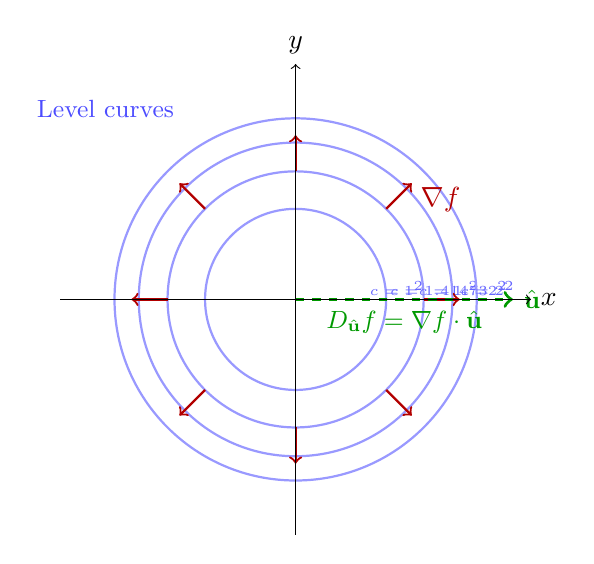
\begin{tikzpicture}[scale=1.15]
  % Draw level curves (circles)
  \foreach \r in {1, 1.414, 1.732, 2} {
    \draw[blue!40, thick] (0,0) circle (\r);
    \node[blue!60, font=\tiny] at (\r+0.12, 0.12) {$c=\r^2$};
  }
  % Gradient vectors (radially outward, proportional to radius)
  \foreach \angle in {0, 45, 90, 135, 180, 225, 270, 315} {
    \pgfmathsetmacro{\px}{cos(\angle)*1.414}
    \pgfmathsetmacro{\py}{sin(\angle)*1.414}
    \pgfmathsetmacro{\dx}{cos(\angle)*0.4}
    \pgfmathsetmacro{\dy}{sin(\angle)*0.4}
    \draw[->, red!70!black, thick] (\px,\py) -- +(\dx,\dy);
  }
  % Label gradient
  \node[red!70!black] at (1.6, 1.1) {$\nabla f$};
  % Directional derivative arrow in direction u=(1,0)
  \draw[->, green!60!black, very thick, dashed] (0,0) -- (2.4, 0)
    node[right, green!60!black, font=\small] {$\hat{\mathbf{u}}$};
  % Projection label
  \node[green!60!black, font=\small] at (1.2, -0.25) {$D_{\hat{\mathbf{u}}}f = \nabla f \cdot \hat{\mathbf{u}}$};
  % Axes
  \draw[->] (-2.6,0) -- (2.6,0) node[right] {$x$};
  \draw[->] (0,-2.6) -- (0,2.6) node[above] {$y$};
  \node[font=\small, blue!70] at (-2.1, 2.1) {Level curves};
\end{tikzpicture}
\end{center}

\subsection*{Figure 2: Surface $z = x^2 + y^2$ with Tangent Plane at $(1,1,2)$}

\begin{center}
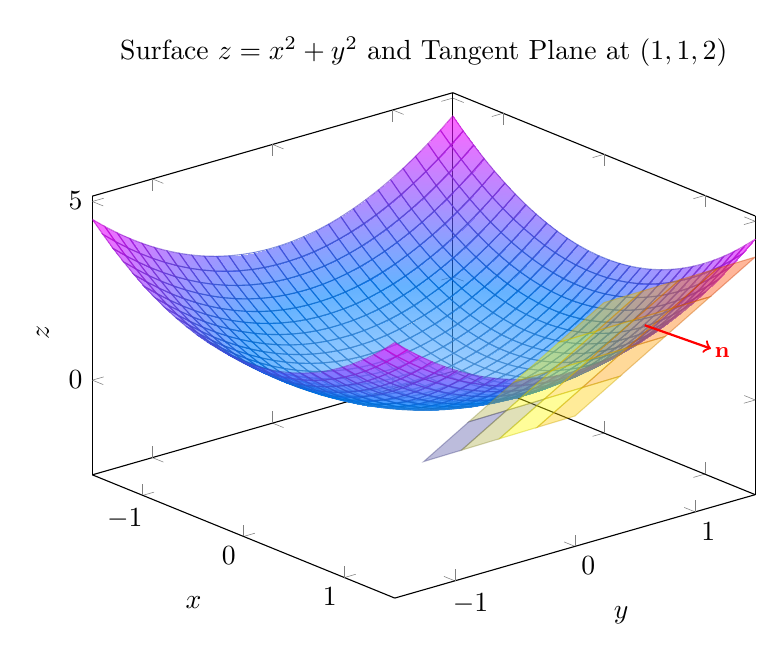
\begin{tikzpicture}
\begin{axis}[
  width=10cm, height=8cm,
  xlabel={$x$}, ylabel={$y$}, zlabel={$z$},
  title={Surface $z=x^2+y^2$ and Tangent Plane at $(1,1,2)$},
  domain=-1.5:1.5, y domain=-1.5:1.5,
  samples=30,
  colormap/cool,
  view={50}{30}
]
  % Paraboloid surface
  \addplot3[surf, opacity=0.6, shader=faceted interp] {x^2 + y^2};
  % Tangent plane: z = 2x + 2y - 2
  \addplot3[surf, opacity=0.4, colormap/hot,
    domain=0:1.5, y domain=0:1.5, samples=5] {2*x + 2*y - 2};
  % Normal vector at (1,1,2)
  \addplot3[->, thick, red, samples y=0]
    coordinates {(1,1,2) (1.3, 1.3, 1.4)};
  \node at (axis cs:1.35, 1.35, 1.3) [red, font=\footnotesize] {$\mathbf{n}$};
\end{axis}
\end{tikzpicture}
\end{center}

\subsection*{Figure 3: Divergence (Source/Sink) and Curl (Rotation) Diagrams}

\begin{center}
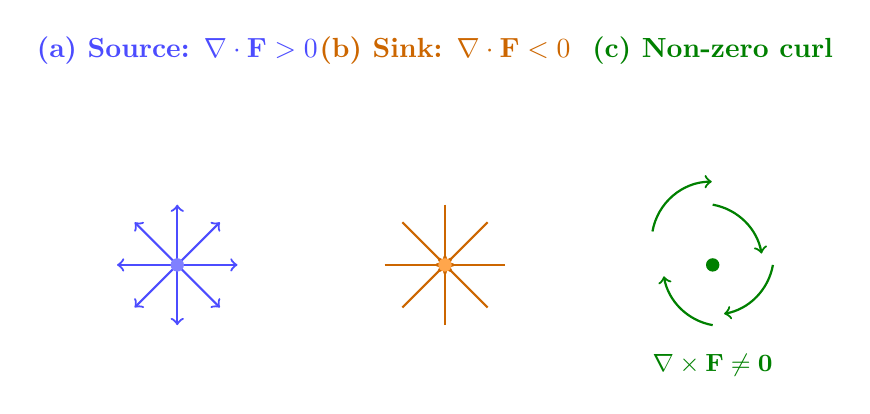
\begin{tikzpicture}[scale=0.85]
  % --- Left: Positive divergence (source) ---
  \node[font=\bfseries, blue!70] at (-4, 3.2) {(a) Source: $\nabla \cdot \mathbf{F} > 0$};
  \foreach \angle in {0, 45, 90, 135, 180, 225, 270, 315} {
    \pgfmathsetmacro{\dx}{cos(\angle)*0.9}
    \pgfmathsetmacro{\dy}{sin(\angle)*0.9}
    \draw[->, blue!70, thick] (-4,0) -- +(\dx,\dy);
  }
  \fill[blue!50] (-4,0) circle (0.1);
  % --- Centre: Negative divergence (sink) ---
  \node[font=\bfseries, orange!80!black] at (0, 3.2) {(b) Sink: $\nabla \cdot \mathbf{F} < 0$};
  \foreach \angle in {0, 45, 90, 135, 180, 225, 270, 315} {
    \pgfmathsetmacro{\dx}{cos(\angle)*0.9}
    \pgfmathsetmacro{\dy}{sin(\angle)*0.9}
    \draw[->, orange!80!black, thick] (-\dx, -\dy) -- (0,0);
  }
  \fill[orange!70] (0,0) circle (0.1);
  % --- Right: Curl (rotation) ---
  \node[font=\bfseries, green!50!black] at (4, 3.2) {(c) Non-zero curl};
  \draw[->, green!50!black, thick] (3.1, 0.5) arc (170:90:0.9);
  \draw[->, green!50!black, thick] (4, 0.9) arc (80:10:0.9);
  \draw[->, green!50!black, thick] (4.9, 0) arc (-10:-80:0.9);
  \draw[->, green!50!black, thick] (4,-0.9) arc (-100:-170:0.9);
  \fill[green!50!black] (4,0) circle (0.1);
  \node[font=\small, green!50!black] at (4,-1.5) {$\nabla \times \mathbf{F} \neq \mathbf{0}$};
\end{tikzpicture}
\end{center}

%==============================================================
\section{Step-by-Step Algorithmic Workflow}
%==============================================================

\begin{infobox}{Seven-Step Workflow for Differential Geometry and Fields}
\begin{enumerate}[leftmargin=*, label=\textbf{Step \arabic*.}]
  \item \textbf{Gradient:} Compute $\partial f/\partial x$, $\partial f/\partial y$, $\partial f/\partial z$ symbolically. Assemble $\nabla f = (f_x, f_y, f_z)$. Substitute the given point to obtain the numerical gradient vector.
  \item \textbf{Directional Derivative:} Identify the direction vector $\mathbf{v}$. Normalise: $\hat{\mathbf{u}} = \mathbf{v}/|\mathbf{v}|$. Compute $D_{\hat{\mathbf{u}}} f = \nabla f \cdot \hat{\mathbf{u}}$ as a dot product (numbers).
  \item \textbf{Tangent Plane (surface $F = 0$):} Write $F(x,y,z) = 0$. Compute $F_x$, $F_y$, $F_z$ and evaluate at $(x_0, y_0, z_0)$. Write $F_x(x - x_0) + F_y(y - y_0) + F_z(z - z_0) = 0$.
  \item \textbf{Normal Line:} From the same point and gradient: $x = x_0 + F_x t$,\; $y = y_0 + F_y t$,\; $z = z_0 + F_z t$.
  \item \textbf{Divergence:} Identify $P$, $Q$, $R$ from $\mathbf{F} = P\mathbf{i}+Q\mathbf{j}+R\mathbf{k}$. Compute $\nabla \cdot \mathbf{F} = \partial P/\partial x + \partial Q/\partial y + \partial R/\partial z$. Check whether result $= 0$ (solenoidal).
  \item \textbf{Curl:} Evaluate the $3 \times 3$ determinant with rows $(\mathbf{i},\mathbf{j},\mathbf{k})$, $(\partial_x, \partial_y, \partial_z)$, $(P, Q, R)$. Note: \textbf{the $\mathbf{j}$ component carries a minus sign.} Check whether result $= \mathbf{0}$ (irrotational).
  \item \textbf{Scalar Potential (if irrotational):} Integrate $\partial \varphi/\partial x = P$ with respect to $x$, obtaining $\varphi = \int P\, dx + g(y,z)$. Differentiate with respect to $y$, match with $Q$ to determine $g$. Differentiate the updated $\varphi$ with respect to $z$, match with $R$ to determine the constant of integration.
\end{enumerate}
\end{infobox}

%==============================================================
\section{Fully Worked Step-by-Step Numerical Examples}
%==============================================================

\subsection*{Example 1: Gradient and Directional Derivative (Basic)}

Let $f(x,y,z) = x^2 y + yz^2$ at $P(1,2,1)$, direction $\mathbf{v} = (1,1,1)$.

\textbf{1.} $f_x = 2xy$,\; $f_y = x^2 + z^2$,\; $f_z = 2yz$.

\textbf{2.} At $P$: $f_x = 4$, $f_y = 2$, $f_z = 4$. So $\nabla f = (4,2,4)$.

\textbf{3.} $\hat{\mathbf{u}} = (1,1,1)/\sqrt{3}$.

\textbf{4.} $D_{\hat{\mathbf{u}}} f = (4+2+4)/\sqrt{3} = 10/\sqrt{3} \approx 5.77$.

\textbf{5.} Maximum rate of increase $= |\nabla f| = \sqrt{16+4+16} = \sqrt{36} = 6$, in direction $(4,2,4)$ or equivalently $(2,1,2)$.

\begin{learnbox}{Key Insight: Example 1}
The directional derivative $10/\sqrt{3} \approx 5.77$ is less than the maximum $6 = |\nabla f|$, confirming $D_{\hat{\mathbf{u}}} f \leq |\nabla f|$. The direction $(1,1,1)$ is not aligned with $\nabla f = (4,2,4)$, hence the reduction.
\end{learnbox}

\subsection*{Example 2: Tangent Plane and Normal Line (Intermediate)}

Find tangent plane and normal line to $x^2 + y^2 + z^2 = 14$ at $(1,2,3)$.

\textbf{1.} Verify: $1 + 4 + 9 = 14$ \checkmark

\textbf{2.} $F = x^2+y^2+z^2-14$. $F_x = 2$, $F_y = 4$, $F_z = 6$ at $(1,2,3)$.

\textbf{3.} Tangent plane: $2(x-1)+4(y-2)+6(z-3)=0 \Rightarrow x+2y+3z=14$.

\textbf{4.} Normal line: $x=1+2t$,\; $y=2+4t$,\; $z=3+6t$.

\begin{learnbox}{Key Insight: Example 2}
The normal direction $(1,2,3)$ is precisely the position vector of the point on the sphere. For any sphere $x^2+y^2+z^2=r^2$, the normal at a point is always radially outward, which is geometrically self-evident.
\end{learnbox}

\subsection*{Example 3: Tangent Plane --- Edge Case (Two Methods)}

Find tangent plane to $z = x^2 + y^2$ at $(1,1,2)$.

\textbf{Method A (explicit):} $z - 2 = 2(x-1) + 2(y-1) \Rightarrow z = 2x + 2y - 2$.

\textbf{Method B (implicit):} $F = x^2+y^2-z$. $F_x=2$, $F_y=2$, $F_z=-1$ at $(1,1,2)$.
\[
2(x-1)+2(y-1)-(z-2)=0 \Rightarrow z = 2x+2y-2 \quad \checkmark
\]

\begin{learnbox}{Key Insight: Example 3}
Converting $z=f(x,y)$ to $F=f-z=0$ always gives $F_z=-1$. The negative sign on $z$ in the implicit form is why the explicit tangent plane uses $z-z_0$ on the left-hand side rather than $z_0-z$.
\end{learnbox}

\subsection*{Example 4: Divergence and Curl (Intermediate)}

$\mathbf{F} = x^2 y\,\mathbf{i} + yz^2\,\mathbf{j} + zx^2\,\mathbf{k}$.

\textbf{Divergence:} $\nabla \cdot \mathbf{F} = 2xy + z^2 + x^2 \neq 0$ in general. \textbf{Not solenoidal.}

\textbf{Curl:}

$\mathbf{i}$: $\partial(zx^2)/\partial y - \partial(yz^2)/\partial z = 0 - 2yz = -2yz$

$\mathbf{j}$: $-[\partial(zx^2)/\partial x - \partial(x^2 y)/\partial z] = -[2xz - 0] = -2xz$

$\mathbf{k}$: $\partial(yz^2)/\partial x - \partial(x^2 y)/\partial y = 0 - x^2 = -x^2$

\[
  \nabla \times \mathbf{F} = -2yz\,\mathbf{i} - 2xz\,\mathbf{j} - x^2\,\mathbf{k} \neq \mathbf{0}
\]

\textbf{Not irrotational.} The field $\mathbf{F}$ is neither solenoidal nor irrotational.

\begin{learnbox}{Key Insight: Example 4}
It is possible for a field to be neither solenoidal nor irrotational simultaneously. Always check both conditions independently --- zero divergence does not imply zero curl, and vice versa.
\end{learnbox}

\subsection*{Example 5: Irrotational Field and Scalar Potential (Applied)}

Verify $\mathbf{F} = 2xyz\,\mathbf{i} + x^2 z\,\mathbf{j} + x^2 y\,\mathbf{k}$ is irrotational. Find $\varphi$ with $\nabla \varphi = \mathbf{F}$.

\textbf{Curl check:} $P=2xyz$, $Q=x^2z$, $R=x^2y$.

$\mathbf{i}$: $R_y - Q_z = x^2 - x^2 = 0$;\quad $\mathbf{j}$: $-(R_x - P_z) = -(2xy-2xy)=0$;\quad $\mathbf{k}$: $Q_x-P_y = 2xz-2xz=0$.

$\nabla \times \mathbf{F} = \mathbf{0}$ \checkmark

\textbf{Potential:} $\varphi = \int 2xyz\, dx = x^2 yz + g(y,z)$.

$\partial \varphi/\partial y = x^2 z + g_y = x^2 z \Rightarrow g_y = 0 \Rightarrow g = h(z)$.

$\partial \varphi/\partial z = x^2 y + h'(z) = x^2 y \Rightarrow h'(z)=0 \Rightarrow h = C$.

$\varphi = x^2 yz + C$.

\begin{learnbox}{Key Insight: Example 5}
The successive integration method works because each step uniquely pins down one unknown function. If at any step a contradiction appears (e.g., $g_y$ depends on $x$), the field is not conservative and no scalar potential exists.
\end{learnbox}

\subsection*{Example 6: Engineering --- Fluid Mechanics (Stagnation Flow)}

Velocity field $\mathbf{V} = 2x\,\mathbf{i} - 2y\,\mathbf{j} + 0\,\mathbf{k}$.

\textbf{Divergence:} $\partial(2x)/\partial x + \partial(-2y)/\partial y + 0 = 2 - 2 = 0$.

$\nabla \cdot \mathbf{V} = 0$ \checkmark \; The fluid is \textbf{incompressible}.

\textbf{Curl:}

$\mathbf{i}$: $\partial(0)/\partial y - \partial(-2y)/\partial z = 0$;\quad
$\mathbf{j}$: $-[\partial(0)/\partial x - \partial(2x)/\partial z] = 0$;\quad
$\mathbf{k}$: $\partial(-2y)/\partial x - \partial(2x)/\partial y = 0$.

$\nabla \times \mathbf{V} = \mathbf{0}$. The flow is \textbf{irrotational}.

\begin{learnbox}{Key Insight: Example 6}
This velocity field describes 2D stagnation-point flow (fluid impinging on a flat wall). Such flows are incompressible \emph{and} irrotational, making them amenable to potential flow theory --- a cornerstone of classical aerodynamics.
\end{learnbox}

%==============================================================
\section{Tabular Reference: Scalar vs Vector Field Operations}
%==============================================================

\begin{center}
\begin{tabular}{>{\bfseries}p{3cm} p{2.5cm} p{1.8cm} p{3.5cm} p{2.5cm} p{2.5cm}}
\toprule
Operation & Input & Output & Formula & Physical Meaning & Engineering Use \\
\midrule
Gradient $\nabla f$ &
Scalar field $f$ &
Vector field &
$\bigl(\partial f/\partial x,\, \partial f/\partial y,\, \partial f/\partial z\bigr)$ &
Direction \& rate of steepest ascent &
Electric field $\mathbf{E} = -\nabla V$ \\[6pt]
Directional Derivative $D_{\hat{\mathbf{u}}} f$ &
Scalar field $f$, unit vector $\hat{\mathbf{u}}$ &
Scalar &
$\nabla f \cdot \hat{\mathbf{u}}$ &
Rate of change in direction $\hat{\mathbf{u}}$ &
Heat flux in a chosen direction \\[6pt]
Tangent Plane &
Surface $F=0$, point &
Plane equation &
$F_x \Delta x + F_y \Delta y + F_z \Delta z = 0$ &
Best linear approximation to surface &
FEM contact patch normal \\[6pt]
Divergence $\nabla \cdot \mathbf{F}$ &
Vector field $\mathbf{F}$ &
Scalar &
$\partial P/\partial x + \partial Q/\partial y + \partial R/\partial z$ &
Source/sink density at a point &
Mass conservation in CFD \\[6pt]
Curl $\nabla \times \mathbf{F}$ &
Vector field $\mathbf{F}$ &
Vector field &
$3\times 3$ determinant form &
Rotational tendency at a point &
Vorticity in fluid flow \\
\bottomrule
\end{tabular}
\end{center}

%==============================================================
\section{Common Student Mistakes and Pitfalls}
%==============================================================

\begin{mistakebox}{Common Mistakes in Differential Geometry and Fields}
\begin{tabular}{>{\bfseries}p{4.2cm} p{4.5cm} p{6.0cm}}
\toprule
\textbf{Mistake Made} & \textbf{Why Students Do It} & \textbf{Correct Mathematical Approach} \\
\midrule
Forgetting to normalise $\mathbf{v}$ before computing directional derivative &
Assume any direction vector can be plugged in directly &
$D_{\hat{\mathbf{u}}} f = \nabla f \cdot \hat{\mathbf{u}}$ requires a \textbf{unit} vector; always divide $\mathbf{v}$ by $|\mathbf{v}|$ first. \\[6pt]
Using $(x, y, z)$ instead of $(x - x_0, y - y_0, z - z_0)$ in the tangent plane &
Copy the formula template without shifting to the specific point &
Tangent plane is $F_x(x-x_0)+F_y(y-y_0)+F_z(z-z_0)=0$; substituting $(x_0,y_0,z_0)$ must give $0=0$. \\[6pt]
Confusing divergence and curl --- applying the scalar formula $\partial P/\partial x + \ldots$ and expecting a vector &
Both involve $\nabla$; students blur the dot and cross product operations &
Divergence $\nabla \cdot \mathbf{F}$ is a \textbf{dot product} and outputs a \textbf{scalar}; curl $\nabla \times \mathbf{F}$ is a \textbf{cross product} and outputs a \textbf{vector}. \\[6pt]
Concluding a field is conservative just because $\nabla \cdot \mathbf{F} = 0$ &
Confusing the solenoidal condition with the irrotational (conservative) condition &
Solenoidal means $\nabla \cdot \mathbf{F} = 0$; irrotational (conservative) means $\nabla \times \mathbf{F} = \mathbf{0}$. These are \textbf{independent} properties. \\[6pt]
Wrong sign on the $\mathbf{j}$ component of curl &
Forgetting that cofactor expansion along the first row gives $(+,-,+)$ signs &
The $\mathbf{j}$ component is $-(\partial R/\partial x - \partial P/\partial z)$; write out the full determinant and apply the correct sign pattern. \\
\bottomrule
\end{tabular}
\end{mistakebox}

%==============================================================
\section{Comprehensive Assessment Suite}
%==============================================================

\subsection*{Viva-Voce Questions (8 questions)}

\begin{enumerate}[leftmargin=*, label=\textbf{Q\arabic*.}]
  \item \textbf{[Gradient]} Define the gradient of a scalar field $f(x,y,z)$. What is the geometric significance of $\nabla f$ at a point?

  \textit{Expected answer:} $\nabla f = (f_x, f_y, f_z)$; it points in the direction of steepest ascent of $f$ and is perpendicular to the level surface $f = c$ through that point.

  \item \textbf{[Directional Derivative]} How is the directional derivative $D_{\hat{\mathbf{u}}} f$ related to the gradient? In which direction is it maximum, and what is that maximum value?

  \textit{Expected answer:} $D_{\hat{\mathbf{u}}} f = \nabla f \cdot \hat{\mathbf{u}}$. It is maximum when $\hat{\mathbf{u}} \parallel \nabla f$, with maximum value $|\nabla f|$.

  \item \textbf{[Directional Derivative]} If $\nabla f = \mathbf{0}$ at a point, what can you say about the directional derivative in any direction at that point?

  \textit{Expected answer:} $D_{\hat{\mathbf{u}}} f = \mathbf{0} \cdot \hat{\mathbf{u}} = 0$ in every direction. The point is a critical point of $f$.

  \item \textbf{[Tangent Plane]} State the equation of the tangent plane to $F(x,y,z) = 0$ at a point. Why is $\nabla F$ normal to the surface?

  \textit{Expected answer:} $F_x(x-x_0)+F_y(y-y_0)+F_z(z-z_0)=0$. Any curve on the surface $F=0$ has its tangent vector satisfying $\nabla F \cdot \mathbf{T} = 0$ (by the chain rule), so $\nabla F$ is perpendicular to every tangent direction.

  \item \textbf{[Tangent Plane]} How do you write the tangent plane to $z = f(x,y)$ at a given point $(x_0, y_0, z_0)$?

  \textit{Expected answer:} $z - z_0 = f_x(x_0,y_0)(x-x_0) + f_y(x_0,y_0)(y-y_0)$.

  \item \textbf{[Divergence/Curl]} Define divergence and curl. State the physical interpretation of each.

  \textit{Expected answer:} $\nabla \cdot \mathbf{F} = P_x+Q_y+R_z$ (scalar) measures the net flux outward per unit volume --- source/sink strength. $\nabla \times \mathbf{F}$ (vector) measures the rotational tendency of the field at that point --- if you placed a paddle wheel there, it tells you the angular velocity of rotation.

  \item \textbf{[Divergence/Curl]} What does it mean for a vector field to be solenoidal? Give one engineering example. What does it mean to be irrotational? Give one engineering example.

  \textit{Expected answer:} Solenoidal: $\nabla \cdot \mathbf{F} = 0$ everywhere (no sources or sinks) --- e.g., incompressible fluid velocity field. Irrotational: $\nabla \times \mathbf{F} = \mathbf{0}$ everywhere (no rotation) --- e.g., static electric field in free space (outside charges).

  \item \textbf{[Divergence/Curl]} State two key vector identities involving gradient, divergence, and curl.

  \textit{Expected answer:} (1) $\nabla \times (\nabla f) = \mathbf{0}$ for any scalar field $f$. (2) $\nabla \cdot (\nabla \times \mathbf{F}) = 0$ for any vector field $\mathbf{F}$.
\end{enumerate}

\subsection*{Descriptive Exam Problems (4 problems)}

\begin{enumerate}[leftmargin=*, label=\textbf{Problem \arabic*.}]
  \item Find the gradient of $f = x^2 yz + 4xz^2$ at the point $(1, -2, -1)$. Find the directional derivative in the direction of $\mathbf{v} = (2, -1, -2)$. Find the maximum rate of change of $f$ at this point and the direction in which it occurs.

  \item Find the equation of the tangent plane and the parametric equations of the normal line to the surface $2xz^2 - 3xy - 4x = 7$ at the point $(1, -1, 2)$. Verify that the point lies on the surface before proceeding.

  \item Let $\mathbf{F} = (x+y+z)\,\mathbf{i} + (x-y+z)\,\mathbf{j} + (x+y-z)\,\mathbf{k}$. Compute $\nabla \cdot \mathbf{F}$ and $\nabla \times \mathbf{F}$. Determine whether $\mathbf{F}$ is solenoidal, irrotational, or neither. If irrotational, find the scalar potential $\varphi$ such that $\mathbf{F} = \nabla \varphi$.

  \item A fluid velocity field is $\mathbf{V} = (x^2 + y^2)\,\mathbf{i} + (y^2 + z^2)\,\mathbf{j} + (z^2 + x^2)\,\mathbf{k}$. Compute $\nabla \cdot \mathbf{V}$ and $\nabla \times \mathbf{V}$. Determine whether the fluid flow is incompressible (solenoidal) and whether it is irrotational. State your conclusions with physical interpretation.
\end{enumerate}

\subsection*{Multiple Choice Questions (6 MCQs)}

\begin{enumerate}[leftmargin=*, label=\textbf{MCQ \arabic*.}]
  \item \textbf{[Gradient]} The gradient $\nabla f$ at a point is perpendicular to:
  \begin{enumerate}[label=(\alph*)]
    \item the $x$-axis
    \item the $y$-axis
    \item \textbf{the level surface $f = \text{constant}$ through that point}
    \item the $z$-axis
  \end{enumerate}
  \textit{Explanation:} $\nabla f$ is always normal to the level surface $f = c$; this is a fundamental geometric property of the gradient.

  \item \textbf{[Directional Derivative]} The directional derivative $D_{\hat{\mathbf{u}}} f$ is maximum when the unit vector $\hat{\mathbf{u}}$ is:
  \begin{enumerate}[label=(\alph*)]
    \item perpendicular to $\nabla f$
    \item opposite to $\nabla f$
    \item \textbf{parallel to $\nabla f$}
    \item any arbitrary direction
  \end{enumerate}
  \textit{Explanation:} $D_{\hat{\mathbf{u}}} f = |\nabla f|\cos\theta$; this is maximised when $\theta = 0$, i.e., $\hat{\mathbf{u}} \parallel \nabla f$.

  \item \textbf{[Tangent Plane]} The vector normal to the surface $F(x,y,z) = 0$ at a given point is:
  \begin{enumerate}[label=(\alph*)]
    \item $\nabla \times \mathbf{F}$
    \item \textbf{$\nabla F$}
    \item $\nabla \cdot \mathbf{F}$
    \item $\partial F/\partial z$
  \end{enumerate}
  \textit{Explanation:} The gradient $\nabla F = (F_x, F_y, F_z)$ is perpendicular to the surface $F = 0$ at every point and defines the tangent plane.

  \item \textbf{[Divergence]} If $\nabla \cdot \mathbf{F} = 0$ everywhere, the vector field $\mathbf{F}$ is called:
  \begin{enumerate}[label=(\alph*)]
    \item irrotational
    \item conservative
    \item \textbf{solenoidal}
    \item harmonic
  \end{enumerate}
  \textit{Explanation:} Solenoidal means zero divergence, implying no net sources or sinks --- the field is divergence-free.

  \item \textbf{[Curl]} If $\nabla \times \mathbf{F} = \mathbf{0}$ everywhere, the vector field $\mathbf{F}$ is called:
  \begin{enumerate}[label=(\alph*)]
    \item solenoidal
    \item \textbf{irrotational}
    \item harmonic
    \item uniform
  \end{enumerate}
  \textit{Explanation:} Zero curl means no rotational component anywhere in the field; the field is irrotational and a scalar potential $\varphi$ exists.

  \item \textbf{[Curl Identity]} For any smooth scalar field $f$, $\nabla \times (\nabla f)$ equals:
  \begin{enumerate}[label=(\alph*)]
    \item $\nabla^2 f$
    \item $\nabla f$
    \item a non-zero vector in general
    \item \textbf{$\mathbf{0}$}
  \end{enumerate}
  \textit{Explanation:} The curl of any gradient is identically the zero vector --- this is an exact vector identity, valid for all smooth scalar fields.
\end{enumerate}

%==============================================================
\section{Quick Recap and Formula Sheet}
%==============================================================

\begin{learnbox}{Differential Geometry and Fields --- Formula Sheet}
\begin{enumerate}[leftmargin=*, label=\textbf{\arabic*.}]
  \item \textbf{Gradient:} $\nabla f = \dfrac{\partial f}{\partial x}\,\mathbf{i} + \dfrac{\partial f}{\partial y}\,\mathbf{j} + \dfrac{\partial f}{\partial z}\,\mathbf{k}$ --- points in the direction of steepest ascent; its magnitude equals the maximum rate of change of $f$.

  \item \textbf{Directional Derivative:} $D_{\hat{\mathbf{u}}} f = \nabla f \cdot \hat{\mathbf{u}}$ --- always use a \textbf{unit} vector $\hat{\mathbf{u}} = \mathbf{v}/|\mathbf{v}|$; maximum value $= |\nabla f|$.

  \item \textbf{Tangent Plane} (implicit surface $F = 0$): $F_x(x-x_0) + F_y(y-y_0) + F_z(z-z_0) = 0$, where $F_x, F_y, F_z$ are partial derivatives of $F$ evaluated at $(x_0, y_0, z_0)$.

  \item \textbf{Normal Line:} $x = x_0 + F_x t,\; y = y_0 + F_y t,\; z = z_0 + F_z t$ --- direction is $\nabla F$ at the point.

  \item \textbf{Divergence:} $\nabla \cdot \mathbf{F} = \partial P/\partial x + \partial Q/\partial y + \partial R/\partial z$ --- scalar; equals zero means solenoidal (incompressible, no sources/sinks).

  \item \textbf{Curl:} $\nabla \times \mathbf{F}$ via the $3 \times 3$ determinant --- vector; equals $\mathbf{0}$ means irrotational (conservative field exists; scalar potential can be found).

  \item \textbf{Key Identity 1:} $\nabla \times (\nabla f) = \mathbf{0}$ always --- every gradient field is irrotational.

  \item \textbf{Key Identity 2:} $\nabla \cdot (\nabla \times \mathbf{F}) = 0$ always --- every curl field is solenoidal.
\end{enumerate}
\end{learnbox}

\end{document}
